\section{Background}
In the past, people may have cited dataset identification numbers explicitly, cited the publication connecting to the dataset's first use, merely mentioned it within a paper, or not cited the dataset at all. Authors and publishers are now encouraged to include data availability information in publications. While much work has focused on PubMed article querying, there still lacks of a unified, systematic way to retrieve datasets.

In 2012, the National Institute of Health launched the Big Data to Knowledge (BD2K) initiative with one of its goals to address poor data accessibility through development of a ``set of platforms and tools by which biomedical researchers can find, reanalyze, and reuse data and which will support data citation metrics and precise scholarly attribution for data''~\cite{bd2k}. One project in particular, bioCADDIE, is developing a Data Discovery Index prototype that aims to have a free, user-friendly means for users to locate data sets of interest. In the long-term, bioCADDIE hopes to be as transformative and impactful for data as PubMed for the biomedical literature~\cite{biocaddie}. The many different use cases and dataset origins proves to be a complication for dataset indexing. For example, a repository may have strict guidelines to only accept primary datasets, not reanalysis, metaanalysis or comparisons. Datasets may also be collected over a range of time, published at various times, or be a subset or derivative of larger, dynamic databases.

To emphasize the current difficulty in searching for datasets, we ask: What is the existing way to search? A direct search requiring background knowledge on the part of the enquirer can be done by searching within a repository for the data or authors directly connected to the dataset. There are also experts who provide searchable lists of curated data sets. The National Institute of Health (NIH) currently manages 65 biomedical data sharing repositories. In the best case, NIH may have invested resources to provide user-friendly mechanisms for query and analysis, such as with GEO. GEO records can be accessed directly using an accession number or queries can be made to study-level or gene-level databases. Queries can be ``effectively performed by simply entering appropriate keywords and phrases into the search box. However, given the large volumes of data stored in these databases, it is often useful to perform more refined queries''~\cite{geoquery}. In other words, efficiently querying requires already knowing what a dataset encompasses.

Finding particular datasets can also be done via MEDLINE citations via the secondary source identifier (SI). Beginning in 2005, many data types discussed within MEDLINE articles, such as sequencing data, gene expression data, and clinical trial data, could be included in the SI element. GEO accession numbers for data started in February 2006; 25 of 38 MEDLINE databank names had 2014 approximate start date to be included in SI field. Fortunately, this means that some dataset indexing can be queried through the NCBI/Entrez databse suite instead of matching regular expression rules, which was done for the DataRank prototype.

The issues with developing a biomedical dataset search engine is similar to what Google faced back in 1998: there is a rapidly growing amount of data leading to a diminishing return effect where retrieval becomes harder as the number and category of datasets increase, the number of users inexperienced in searching for relevant data sets increases, and the mental resources to parse through search results decrease. All this hints for the need of higher precision when targeting or personalizing results as the search space grows. Citation analysis and bibliometrics establish precedence of ideas and hint at the quality or significance of a scientific work. We apply these ideas to learn about datasets with the end goal of developing a personalized biomedical dataset search engine. 

The networks arising from PubMed/MEDLINE citations are inherently hetergeneous: multiple objects types have interactions with other types based on different relations. For example, researchers may cite others via journal publications, papers may belong to different topical areas, datasets may be shared and reanalyzed for different papers, and authors may be socially connected by collaboration, citation, or organizations. Figure~\ref{fig:hetero} shows an example of the object types and relations we explore with PubMed.

\begin{figure}[h]
    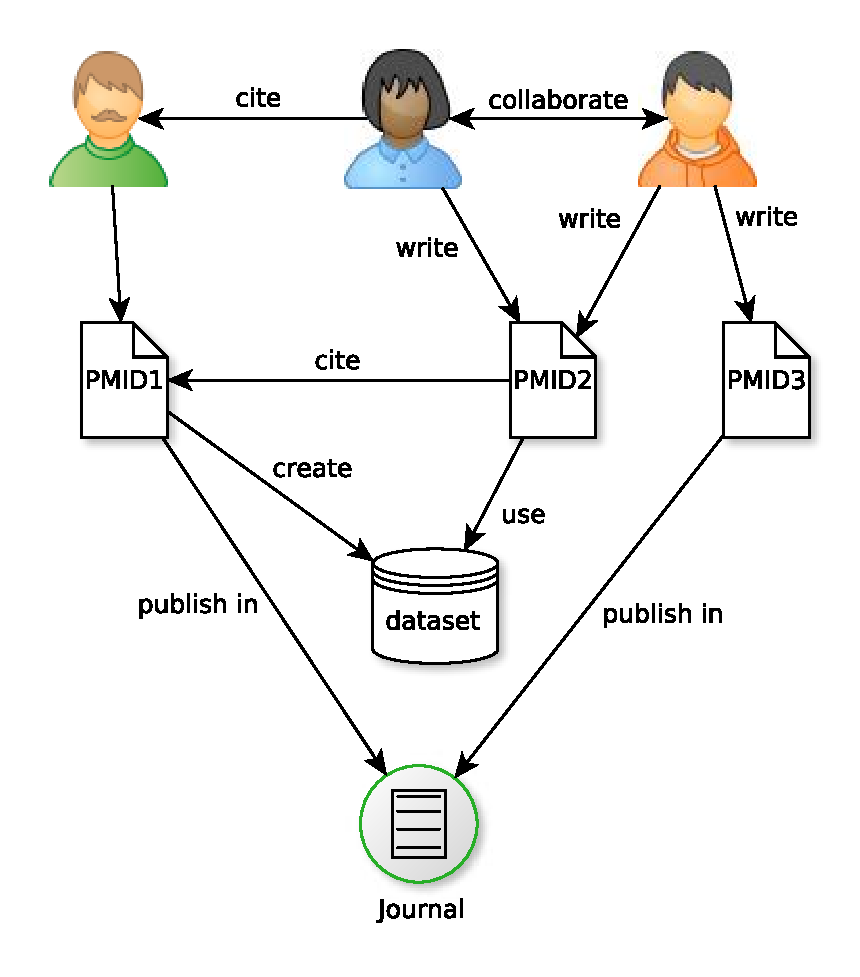
\includegraphics[width=\columnwidth]{hetero.eps}
    \caption{Small Heterogeneous Network}
    \label{fig:hetero}
\end{figure}